\documentclass[11pt]{beamer}
\usepackage[utf8]{inputenc}
\usepackage[T1]{fontenc}
\usepackage[english,russian]{babel}
\include{metropolis/*.sty}
\usetheme{metropolis}
\title{TeXstudio}
\date{\today}
\begin{document}
	\maketitle
	\begin{frame}{TeXstudio}
		\begin{columns}[c,onlytextwidth]
			\begin{column}{0.44\textwidth}
					«TeXstudio» -- кросс-платформенный редактор \text{\LaTeX} с открытым кодом, подобный Texmaker.
					TeXstudio распространяется без пакета \text{\LaTeX} -- пользователь должен самостоятельно выбрать и установить нужный дистрибутив \text{\LaTeX}.  
			\end{column}
			\begin{column}{0.50\textwidth}
				\begin{figure}
					\centering
					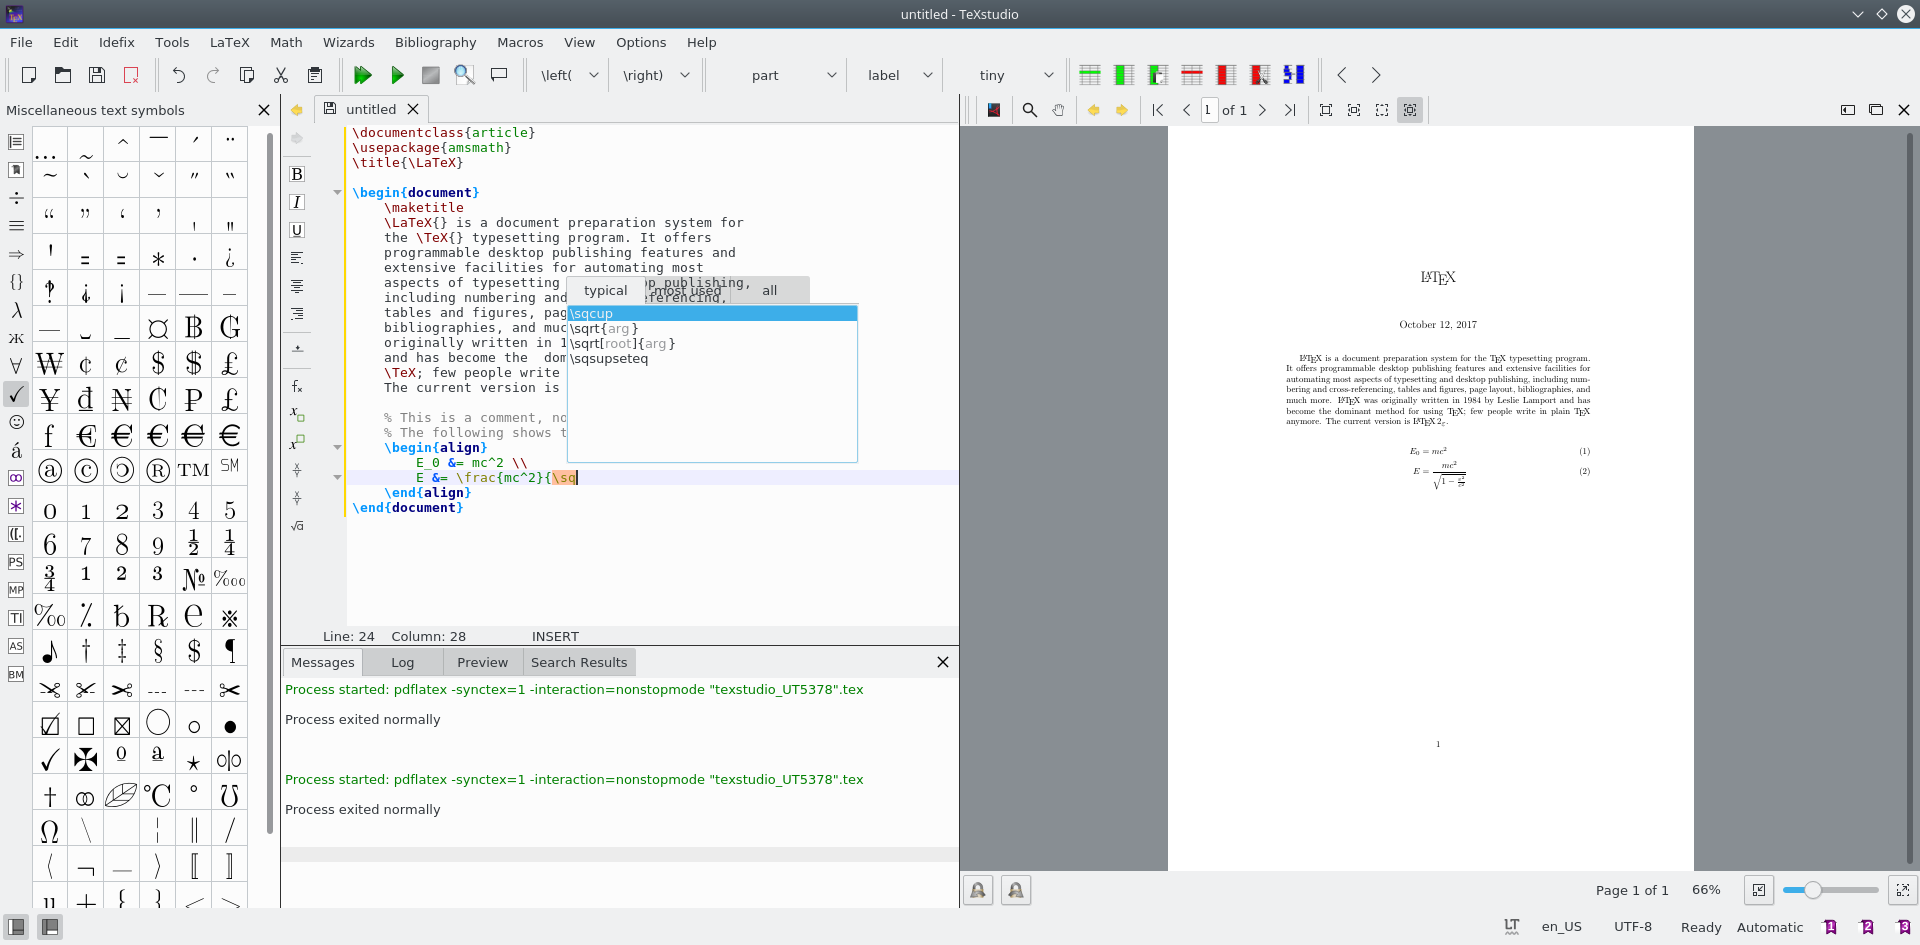
\includegraphics[width=\textwidth]{res/TeXstudio.png}
				\end{figure}
				\begin{figure}
					\centering
					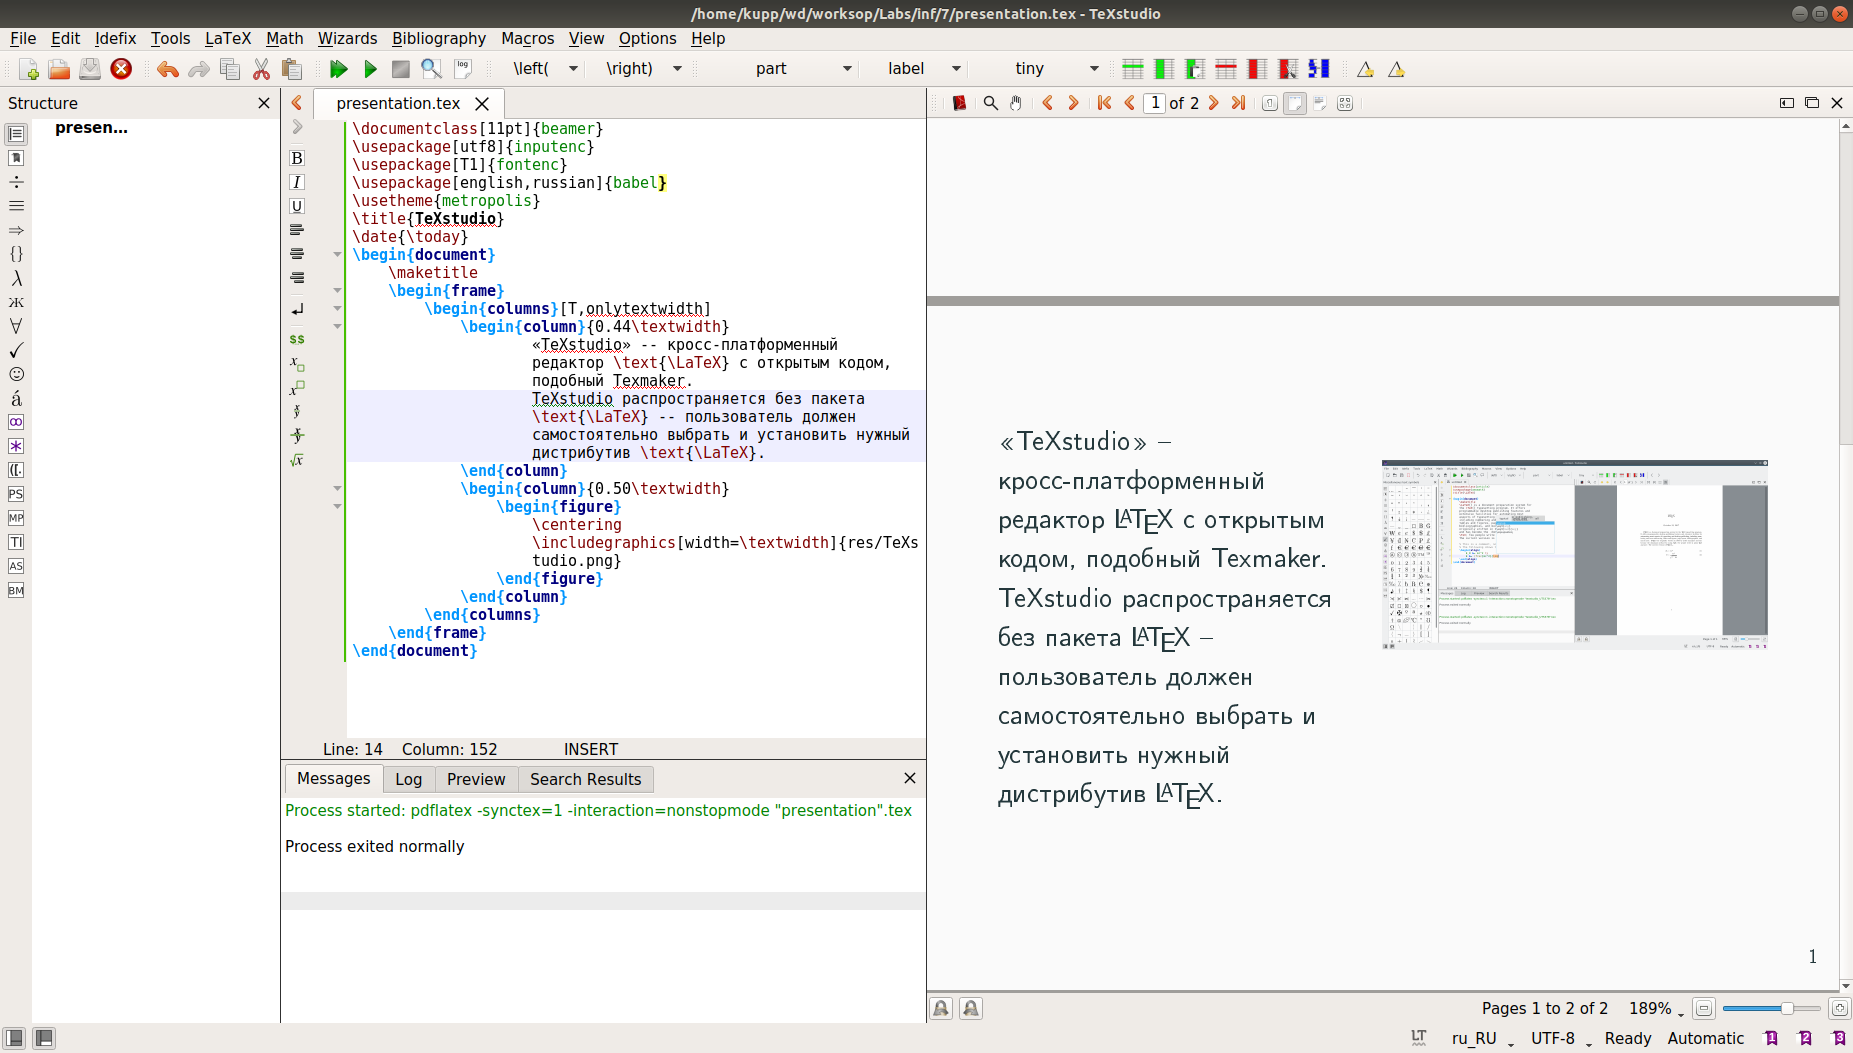
\includegraphics[width=\textwidth]{res/myscreen.png}
				\end{figure}
			\end{column}
		\end{columns}
	\end{frame}
	\begin{frame}{История}
		\begin{columns}[c,onlytextwidth]
			\begin{column}{0.44\textwidth}
				TeXstudio возник как ответвление от Texmaker в 2009 году, в силу закрытого процесса разработки Texmaker и разной философии. Сначала он назывался TeXmakerX, потому что разрабатывался как маленький набор расширений к Texmaker с надеждой на то, что они когда-нибудь будут интегрированы в Texmaker.
			\end{column}
			\begin{column}{0.50\textwidth}
				\begin{figure}
					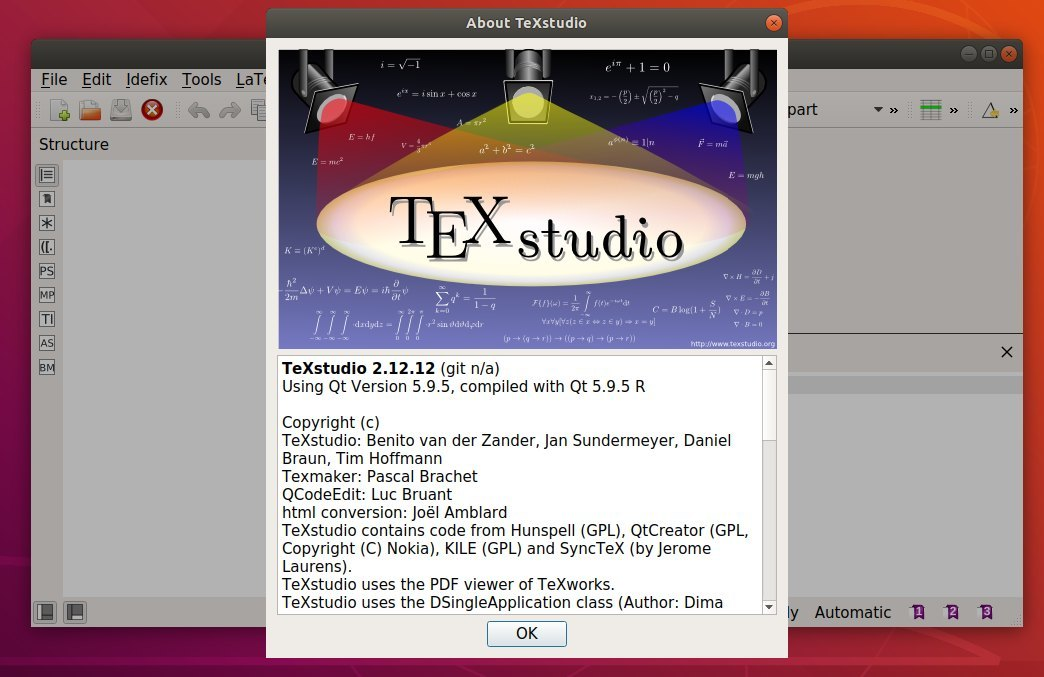
\includegraphics[width=\textwidth]{res/texstudio21212.jpg}
				\end{figure}
			\end{column}
		\end{columns}
	\end{frame}
	\begin{frame}{Возможности}
		\begin{columns}[c,onlytextwidth]
			\begin{column}{0.70\textwidth}
				\begin{itemize}
					\item Подсветка синтаксиса
					\item Проверка правописания
					\item Интегрированный просмотрщик PDF
					\item Поддержка написания скриптов
					\item Мастер для рисунков, таблиц, формул
				\end{itemize}
			\end{column}
			\begin{column}{0.25\textwidth}
				\begin{figure}
					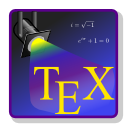
\includegraphics[width=\textwidth]{res/Texstudio_Logo.png}
				\end{figure}
			\end{column}
		\end{columns}
	\end{frame}
\end{document}